\documentclass{article}
\usepackage{graphicx}
\usepackage{float}
\usepackage{gensymb}
\parskip=12pt

\begin{document}

\title{Laboratory 6: Diffraction and Interference}
\date{December 12, 2014}
\author{Calvin Chan\\304144970\\Physics 4BL Lab 8\\Partners: Caleb Choi, Stanley
Chan}

\maketitle

\section{Introduction}

This lab explores light interference and demonstrates the duality of light as,
both, a wave and a particle. It attempts to prove the validity of several
equations that govern electromagnetic waves. By measuring the interference
patterns of light through various medium (single slit, double slits, diffraction
grating, and hair), we can show how these electromagnetic waves constructively
and destructively interfere with each other.

\section{Experimental Results}

Using an optic fiber cable connected to a photometer, we were able to measure
the light intensity of laser patterns. By shining a laser through two slits, we
could create an interference pattern through diffraction. By moving the
photometer sensor through the bright and dark fringes, we can record the
corresponding voltage of each fringe. To start, we had to calibrate the
potentiometer by determining the conversion factor between voltage and position
by recording the intensity of a flat laser beam with no diffraction, as shown in
fig. \ref{calibration}.

\begin{figure}[H]
    \centering
    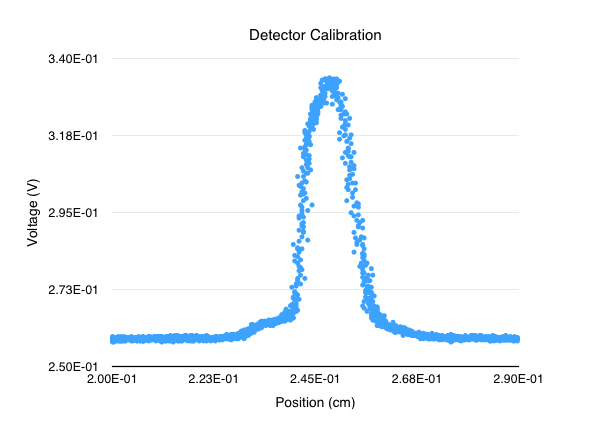
\includegraphics[width=\textwidth]{charts/calibration}
    \caption{Using a linear laser beam to calibrate for a position/voltage
    conversion}
    \label{calibration}
\end{figure}

Evidently, the intensity is the greatest at the middle, exactly where the laser
beam hits the sensor, and fades out the further away from the beam center the
sensor is. Using the highest recorded voltage and the lowest recorded voltage,
we find the difference in voltages and divide it by the distance the sensor
moved. We can then use this conversion factor for the rest of our experiments to
convert our voltage measurements into position measurements (cm).

For our experiment, our conversion factor was $0.474531 \frac{cm}{V}$.

\subsection{Double-slit diffraction}

\begin{figure}[H]
    \centering
    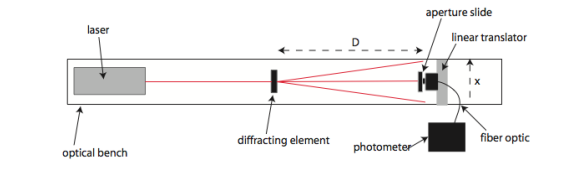
\includegraphics[width=\textwidth]{charts/double-slit}
    \caption{Setup for double slit diffraction experiments}
    \label{double-slit}
\end{figure}

After calibration, we took a double slit grating with known parameters and
placed it in line with the laser beam, such that the beam shined through the
grating and diffracted onto the sensor. Using the conversion factor from the
previous part of the lab, we were able to convert the voltage measurements of
the position channel to reflect the actual position of the center in
centimeters. This is represented in the following figure.

\begin{figure}[H]
    \centering
    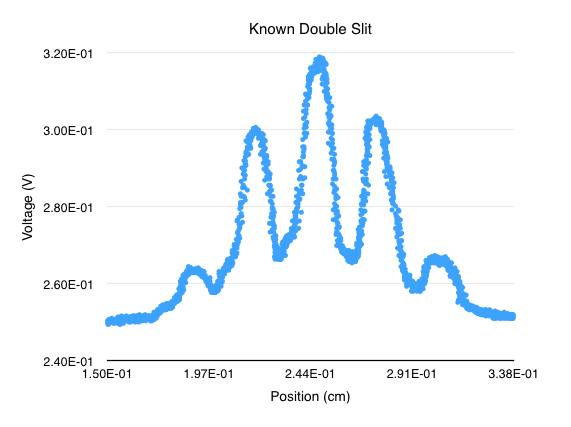
\includegraphics[width=0.8\textwidth]{charts/known}
    \caption{Using a linear translator for the position/voltage conversion}
    \label{known}
\end{figure}

We then repeated the experiment with three different double slit gratings, with
unknown parameters. This is represented in the following figures.

\begin{figure}[H]
    \centering
    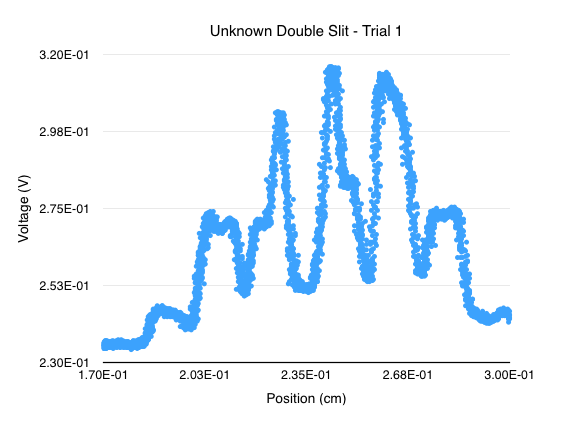
\includegraphics[width=0.8\textwidth]{charts/unknown1}
    \caption{Using a linear translator for the position/voltage conversion}
    \label{unknown1}
\end{figure}

\begin{figure}[H]
    \centering
    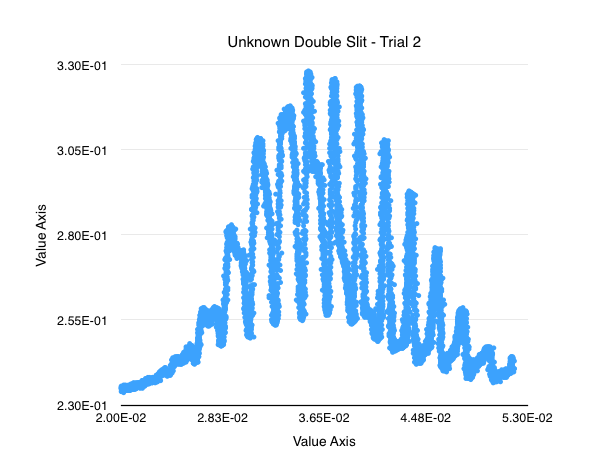
\includegraphics[width=0.8\textwidth]{charts/unknown2}
    \caption{Using a linear translator for the position/voltage conversion}
    \label{unknown2}
\end{figure}

\begin{figure}[H]
    \centering
    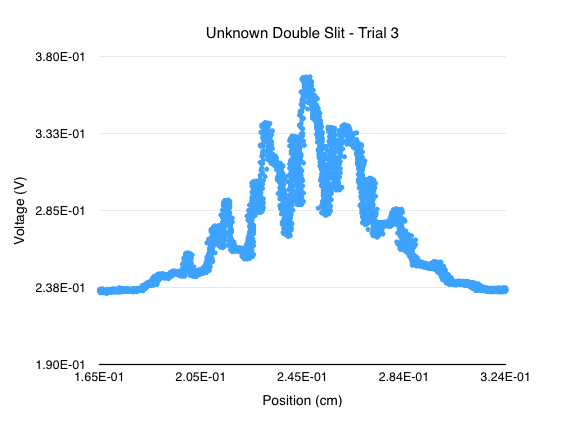
\includegraphics[width=0.8\textwidth]{charts/unknown3}
    \caption{Using a linear translator for the position/voltage conversion}
    \label{unknown3}
\end{figure}

\subsection{Diffraction Grating}

This part of the lab further demonstrates the diffraction properties of light
and how light behaves due to diffraction. By shining a laser through a
diffraction grating, we were able to use a protractor to measure the diffraction
angles of the light as it traveled through the grating. The following chart
shows the angles of the maxima that we recorded.

\begin{figure}[H]
    \centering
    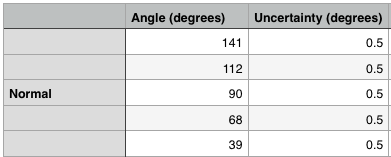
\includegraphics[width=0.8\textwidth]{charts/diffraction-grating}
    \caption{The recorded maxima of a laser shined through a diffraction grating}
    \label{diffraction-grating}
\end{figure}

\subsection{Dispersion of White Light}

We then proceeded to repeat the previous step of the experiment with white light
instead of a laser. We used a white light ray box and a filter to create one
ray. We shined that ray through the diffraction grating and measured the
principle colors and their diffraction angles through the grating. The following
chart shows what was achieved.

\begin{figure}[H]
    \centering
    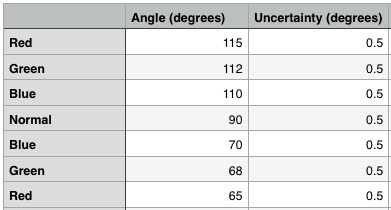
\includegraphics[width=0.8\textwidth]{charts/dispersion-white-light}
    \caption{The dispersion of white light into different principle colors}
    \label{dispersion-white-light}
\end{figure}

\subsection{Other scatterer - Hair strand}

Finally, we repeated the dispersion experiment again, shining a laser beam
against the hair and observing the single-slit diffraction pattern as the beam
traveled through the hair and onto a white piece of paper. The following chart
shows the maxima and minima locations (measured from the center) of the
diffraction pattern.

\begin{figure}[H]
    \centering
    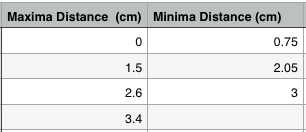
\includegraphics[width=0.55\textwidth]{charts/human-hair}
    \caption{The recorded maxima and minima of a laser shined through a strand
    of human hair}
    \label{human-hair}
\end{figure}

\section{Analysis}

To determine the voltage/position conversion factor, we use the following
formula to compare the change in voltage with the change in position, with error
propogation calculated as well.

\begin{equation}
    \label{vp-conversion-1}
    m = \frac{\bigtriangleup x}{\bigtriangleup V} = 0.474531 \frac{cm}{V}
\end{equation}
\begin{equation}
    \label{vp-conversion-2}
    \sigma_{m} = \frac{\sigma_{\bigtriangleup x}}{\bigtriangleup V} = 0.007924
    \frac{cm}{V}
\end{equation}

\subsection{Double-slit diffraction}

Using the following formula (eq. \ref{double-slit-eq}), we can calculate the
slit width and spacing.

\begin{equation}
    \label{double-slit-eq}
    d sin\theta = m\lambda
\end{equation}

With small angle approximations, we can assume that $sin\theta = tan\theta$,
which gives us the following:

\begin{equation}
    \label{double-slit-eq-2}
    d = \frac{m\lambda D}{x}
\end{equation}

Using equation \ref{double-slit-eq-2}, we can calculate the slit spacing for
each trial of the double slit diffraction experiment, as shown in the following
charts.

\begin{figure}[H]
    \centering
    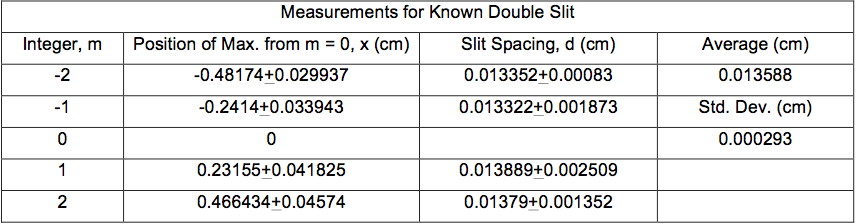
\includegraphics[width=\textwidth]{charts/known-chart}
    \caption{Slit spacing for the known double slit grating}
    \label{known-chart}
\end{figure}

By averaging the calculated split spacing, we can compare it to the value of the
actual split spacing, $0.0125 cm$.

\begin{equation}
    \label{percent-error-split-spacing}
    percent error = \frac{0.0135-0.0125}{0.0125} = 8.70\%
\end{equation}

However, we can see that our calculated split spacing lies outside of the errors
for the actual value.

\begin{figure}[H]
    \centering
    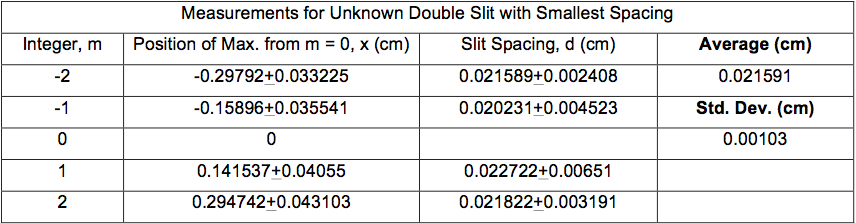
\includegraphics[width=\textwidth]{charts/unknown-chart-1}
    \caption{Slit spacing for one of the unknown double slits}
    \label{unknown-chart-1}
\end{figure}

\begin{figure}[H]
    \centering
    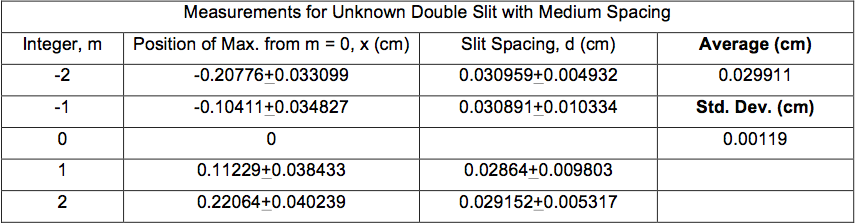
\includegraphics[width=\textwidth]{charts/unknown-chart-2}
    \caption{Slit spacing for the second of the three unknown double slits}
    \label{unknown-chart-2}
\end{figure}

\begin{figure}[H]
    \centering
    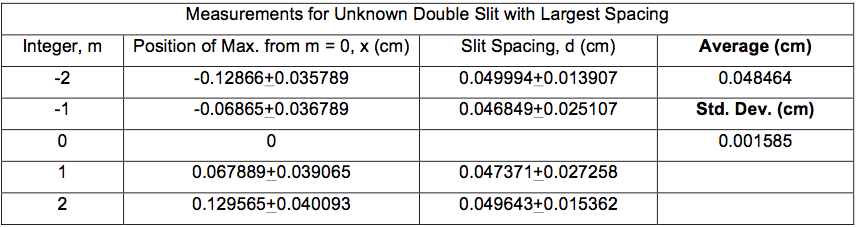
\includegraphics[width=\textwidth]{charts/unknown-chart-3}
    \caption{Slit spacing for the third unknown double slit}
    \label{unknown-chart-3}
\end{figure}

It is easily observable that the space between adjacent maxima decreases as the
slit spacing increases.

Furthermore, we can calculate the slit width of a double slit using a similar
approach. Using a component of intensity that is dependent on the slit width, we
can use the following equation to determine the slit width, b, of the largest
unknown slit.

\begin{equation}
    \label{slit-width-1}
    sin(\frac{\pi b sin\theta}{\lambda}) = 0
\end{equation}
\begin{equation}
    \label{slit-width-2}
    \frac{\pi b sin\theta}{\lambda} = \pi 
\end{equation}
\begin{equation}
    \label{slit-width-3}
    b tan\theta = \lambda
\end{equation}
\begin{equation}
    \label{slit-width-4}
    b = \frac{l\lambda}{y} = 0.003761 \pm 0.000242 cm
\end{equation}

\subsection{Diffraction grating}

Using equation \ref{diffraction-grating-eq-1} and a wavelengthof $670 nm$, we
can verify the validity of the slit spacing in the diffraction grating.

\begin{equation}
    \label{diffraction-grating-eq-1}
    d sin\theta = n\lambda
\end{equation}

The following chart shows the calculated value of the slit spacing through the
diffraction grating.

\begin{figure}[H]
    \centering
    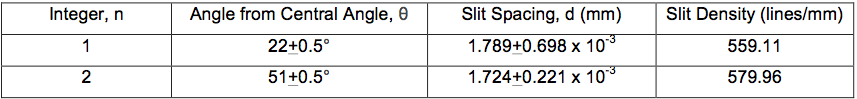
\includegraphics[width=\textwidth]{charts/diffraction-grating-chart}
    \caption{Slit spacing due to diffraction grating}
    \label{diffraction-grating-chart}
\end{figure}

By averaging the two calculated slit densities, we obtain an average slit
spacing of $567.5 lines/mm$. We can see that this is within the acceptable
errors by comparing slit spacing values.

\begin{equation}
    \label{percent-error-diffraction-grating}
    percent error = \frac{600-567.5}{600} = 5.12\%
\end{equation}

\subsection{Dispersion of White Light}

Similarly, we can calculate the wavelength of each color of light after the
dispersion of the white ray through the dispersion grating using the following
formula.

\begin{equation}
    \label{dispersion-white-light}
    \lambda = sin\theta d
\end{equation}

The following chart shows the results of our calculations.

\begin{figure}[H]
    \centering
    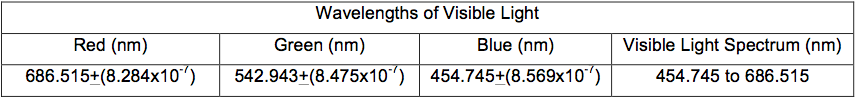
\includegraphics[width=\textwidth]{charts/white-dispersion-chart}
    \caption{Wavelengths of the principal colors due to dispersion}
    \label{white-dispersion-chart}
\end{figure}

Using acceptable wavelength values for red light (620-720nm), blue light
(450-495nm), green light (495-570nm), and the visible light spectrum
(390-700nm), it is shown that our calculations are within the acceptable
ranges.

\subsection{Other scatterer - Hair strand}

Using equation \ref{double-slit-eq-2}, the thickness of the hair strand can be
calculated as well. With an average distance between adjacent maxima of $7.05
\pm 0.05 cm$, it can be calculated that the thickness of a single strand of
human hair is $7.6066 \pm 0.0553 * 10^{-4} cm$. Comparing to a standard human
hair thickness of between $10^{-6} cm$ and $10^{-3}$, it can be said that our
calculations lie within the acceptable range and are valid.

\section{Conclusion}
This experiment demonstrated the various behaviors and properties of light
through diffraction and interference. We demonstrated the behavior of light
through double slits, and how light diffraction is caused by light traveling
through double slits. Although our calculated value for the known split spacing
was not within the error bounds acceptable for that particular measurement, we
were very close and could attribute the error to human errors in calibration and
placement of equipment. For the diffraction grating, we demonstrated the
behavior of light shining through multiple slits. Additionally, we were able to
observe the principla colors of the visible spectrum of light by shining a white
ray beam into the diffractiong rating. Finally, we showed that something as
simple as a strand of hair is capable of causing light diffraction.
\end{document}
